
\chapter{Introduction}

\begin{itemize}
	\item Kubernetes abstracts away the hardware infrastructure and exposes your whole data-center as a single enormous computational resources.
	\item To reduce the number of problems that only show up in production, it would be ideal if applications could run in the exact same environment during development and in production so they have the exact same operating system, libraries, system configuration, networking environment, and everything else.
	\item Ideally, you want the developers to deploy applications themselves without knowing anything about the hardware infrastructure and without dealing with the ops team.
	\item container technologies
	\item When using containers, you can (and should) have one container for each application.
	\item Linux Namespaces
	\item Linux Control Groups (cgroups)
	\item Kubernetes enables you to run your software applications on thousands of computer nodes as if all those nodes were a single, enormous computer.
	\item Kubernetes will expose all of them at a single static IP address and expose that address to all applications running in the cluster. This is done through environment variables.
	\item The IP address of the service stays constant, so clients can always connect to its containers, even when they're moved around the cluster.
	\item On any node where Kubernetes is deployed, Kubernetes can run the app immediately without any help from the sysadmins.
\end{itemize}


\section{Features}
\begin{itemize}
	\item service discovery
	\item auto scaling
	\item load balancing
	\item self-healing
	\item leader election
\end{itemize}

\section{Concepts}

\begin{itemize}
	\item master node
	\item Kubernetes Control Planes
	\item worker node
\end{itemize}



\section{Kubernetes Cluster Architecture}

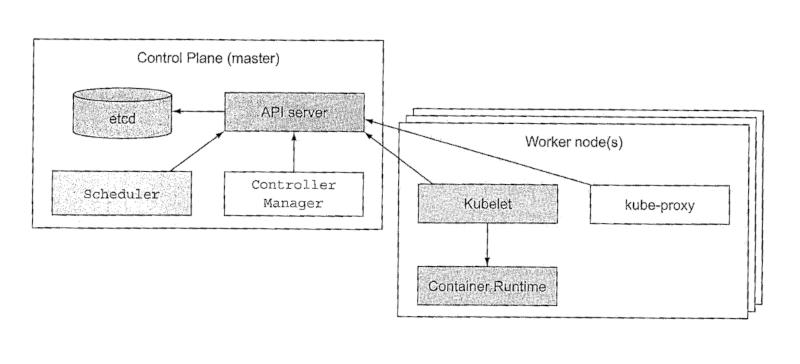
\includegraphics[max width=\textwidth]{introduction/k8s_cluster_architecture.png}